\documentclass[12pt]{article}
\usepackage{graphicx}

\begin{document}

Andrew Brandt
9-4-2022

\Large 01 Puzzle 2 - The Lanterns of Lumenville

\vspace{5mm}

\noindent
\vspace{5mm}
\large Puzzle:

Lumenville is a decidedly strange village. It consists of 36 cubical, single room houses with
glass walls arranged in a square grid with narrow paths running by each house.
The Lumenarians who inhabit Lumenville are even more strange. They are incredibly nosey,
hence the requirement in the city charter that all houses have glass walls, but intensely private as
well, so only one Lumenarian can live in each house. There are exactly 36 Lumenarians, always
has been, always will be.

\vspace{5mm}

The Lumenarians are also famously frugal to a fault. They watch their phots with great
vigilance. This was shown at a recent city council meeting, a virtual meeting, of course. The
Luminarie who lives in house Three-and-Three, who always acted like they were near the the
center of the Lumenarian Universe, proposed that a lantern be placed in each Lumenville house
so everyone could be nosey at night as well as in the day. But when approval of the purchase
order to the Luminous Lantern Ltd company came up for approval there was an uproar. Thirtysix lanterns, it said, at a total cost of 360 phots, one for every Lumenville house.
Objections came fast and furious. “Why do I need to pay for a lantern”, said the occupant of
house One-and-Three. “I live at the west edge of town and my house will be illuminated by any
of my neighbors to the north, south, east or north-east or south-east. Let one of those 15
Luminarians buy a lantern. I will help pay for it, of course, but not a phot more than I absolutely
have to.”

\vspace{5mm}

Tumult and commotion reigned as each Lumenarian claimed the same privilege. But clearly
someone had to buy a lantern. But how can we determine who needs to buy a lantern so the
frugal tendencies of the Lumenarians are appeased and how many phots it will take?
Just to illuminate the details of the situation, note that a lantern only illuminates houses along
lines east-west and north-south and along the two diagonals in between. And to further clarify, a
lantern in a corner glass house fully illuminates 16 houses.
Now, if you are simply trying different lantern positions over and over and over and over and
over and over hoping to find a solution to this puzzle it might occur to you to try to determine
instead the number of lanterns you would have to place in the houses to illuminate every house
no matter where you put them. Find a solution to this version of the puzzle too.


\vspace{100mm}

\center Model of village:

\vspace{5mm} %5mm vertical space

\center{
\includegraphics[scale=.5]{36 grid}}

\vspace{5mm}
\center{
\includegraphics[scale=.1]{comapssrose}}
\noindent 

\vspace{10mm}

a lantern only illuminates houses along lines east-west and north-south and along the two diagonals in between

\vspace{5mm}
The only way I can think to solve this at first is just by using brute force. If I find a solution I will recognize it.

\vspace{5mm}


\center{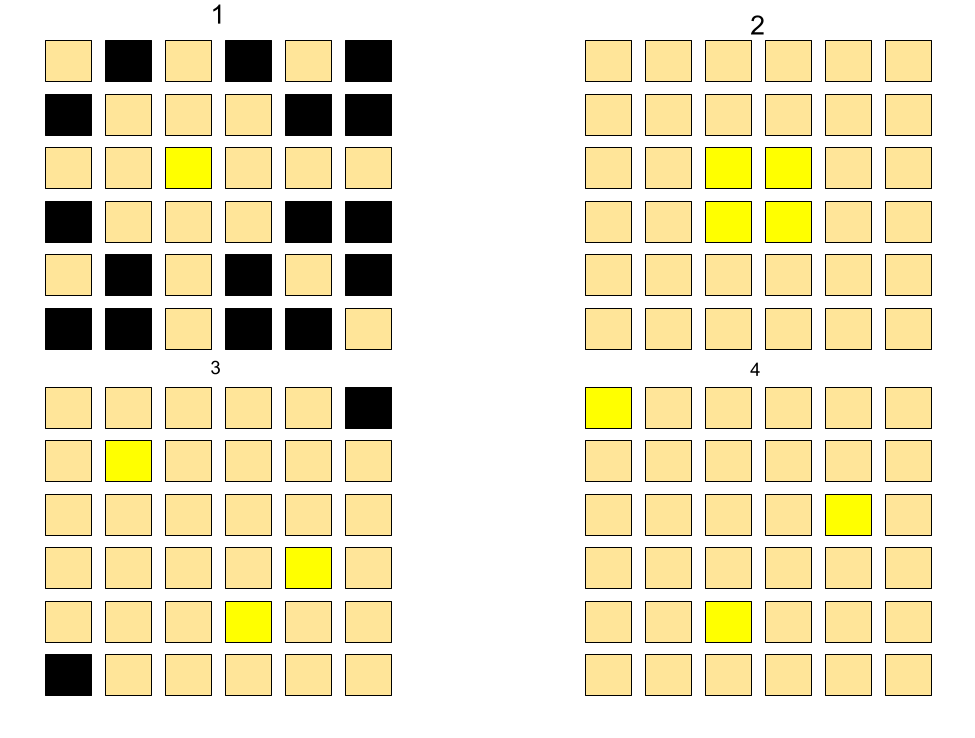
\includegraphics[scale=.4]{lightex}}

Note: The yellow squares are houses with lanterns and the tan are houses that are lit up as a result of the lantern placement.

\vspace{5mm}

From my tests and drawings, the least amount of lanterns that I could use to light up all the houses was 3.
There may be a way to do all of them with 2, but I have not found that solution yet.

\vspace{5mm}
I believe that placing 5 lanterns or more anywhere on the grid will result in the entire village being lit up.
Placeing 4 lanterns and lighting up the village is a fairly easy thing to do, but there are certain placements that do not result in every house having light.

\vspace{5mm}
The solution presented in example 4 above gives light to every house with a total of 3 lanterns. The problem with this is that there is much overlap between the two at the bottom of the grid.
Assuming the cost of 10 phots per lantern, the total cost is 30 phots or a little less that a phot per inhabitant.

\end{document}
